% ----------------------------------------------------------
% Introdução
% ----------------------------------------------------------
\chapter[\label{ch:intro}Introdução]{Introdução}
Aqui vai o texto da introdução.  

A ABNT indica a elaboração de uma lista de ilustrações com todos os itens arrolados e designados por seu nome específico, conforme a ordem que aparecem no texto (Figura 1, Fotografia 1, Gráfico 1, Quadro 1, entre outros). Também recomenda, quando necessário, a elaboração de lista própria para cada tipo de ilustração. No entanto, não determina um número mínimo de ilustrações para tal lista específica.

\section{\label{sec:tema}Tema}

escreva aqui...

\subsection{\label{sec:deltema}Delimitação do tema}
Aqui vai a delimitação do tema se tiver descrito na seção~\ref{sec:tema}.




\section{\label{sec:probPesquisa}Problema}
escreva aqui...

\section{\label{sec:objGeral}Objetivo geral}
escreva aqui...

\subsection{\label{sec:objEsp}Objetivos Específicos}
\begin{enumerate}
	\item objetivo especifico aqui...
	\item objetivo especifico aqui...
\end{enumerate}

\section{\label{sec:just}Justificativa}
escreva aqui...

\chapter[\label{ch:ref}Referencial Teórico]{Referencial Teórico}
aqui vai o texto do referencial teórico. 

Vc deve inserir novas seções e subseções. Recomendo usar labels para todas as seções.

\section{\label{sec:citacao}Citações}

Este parágrafo serve apenas para explicar as citações de referências. 

Os dois parágrafos a seguir mostram, respectivamente, como fazer uma citação indireta e direta. 

Conforme~\citeauthoronline{bourg2013physics}, o quadrado não é redondo e o círculo não é quadrado. Esta próxima citação é do tipo direta, onde copiamos uma frase inteira do autor. 

Poderíamos refletir sobre a "existência de quadrados redondos e círculos quadrados"~\cite{ericson2004real}. 


\subsection{\label{subsec:citacaoLonga}Citação longa}

O texto abaixo demonstra uma citação direta com mais de 3 linhas. Segundo~\cite{ericson2004real}:

\begin{citacao}
	O texto deve ser constituído de uma parte introdutória, na qual devem ser
	expostos o tema do projeto, o problema a ser abordado, a(s) hipótese(s),
	quando couber(em), bem como o(s) objetivo(s) a ser(em) atingido(s) e a(s)
	justificativa(s). É necessário que sejam indicados o referencial teórico que
	o embasa, a metodologia a ser utilizada, assim como os recursos e o cronograma
	necessários à sua consecução.
\end{citacao}


\section{\label{sec:quadros}Uso de quadros para códigos}

Quadro é um espaço não afetado pelas formatações do latex. O quadro aceita apenas texto em UTF-8 (textos com caracteres especias precisam de outra solução).

A referencia~\cite{ericson2004real} é retirada de um livro, enquanto a referência~\cite{Silverman20201569} é de um artigo. O tipo de publicação é informado no arquivo \emph{bibliografia.bib}. 

O quadro~\ref{lst:quadro1} mostra um exemplo de referencia armazenada no arquivo das \emph{bibliografia.bib}.

\begin{lstlisting}[caption={Exemplo referência},label={lst:quadro1}]
@ARTICLE{Silverman20201569,
	author = {Silverman, Linda K. and Gilman, Barbara J.},
	title = {Best practices in gifted identification and assessment: 
		Lessons from the WISC-V},
	year = {2020},
	journal = {Psychology in the Schools},
	volume = {57},
	number = {10},
	pages = {}1569 - 1581},
	doi = {10.1002/pits.22361},
	url = {https:/link.com.br},
	type = {Article},
	publication_stage = {Final},
	source = {Scopus},
	note = {Cited by: 14}
}
\end{lstlisting}
	

\section{\label{sec:ilustrações}Ilustrações}
Este parágrafo serve apenas para explicar como é inserido uma imagem. Não devem existir figuras não referenciadas no corpo do texto. A Figura~\ref{fig:figura1} mostra duas formas geométricas, enquanto a Figura~\ref{fig:figura2} mostra o diagrama de uma arquitetura imaginária de autoria própria.

\begin{figure}[htb]
	\centering
	\caption{\label{fig:figura1} Figura apresentando uma representação gráfica de uma esfera a esquerda e um cubo a direita.}
	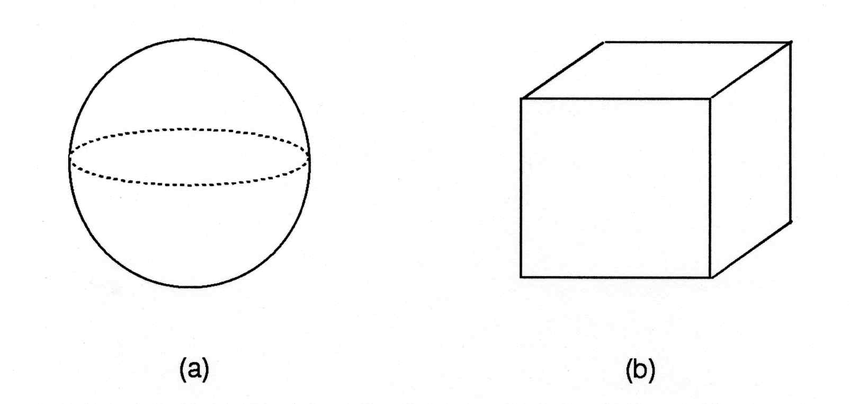
\includegraphics[width=\textwidth]{imgs/figura1.png}
	\legend{Fonte: \cite{bourg2013physics}.}
\end{figure}

No campo $\backslash$caption vai a label da figura (que é única em todo texto ) e a descrição da figura (chamamos de legenda). No campo $\backslash$legenda vai a fonte, informando a origem da figura. A instrução $\backslash$centering faz com que os elementos sejam centralizados.


\begin{figure}[htb]
	\centering
	\caption{\label{fig:figura2} Arquitetura imprevista: um sistema projetado para um projeto de pesquisa que pesquisaria algo.}
	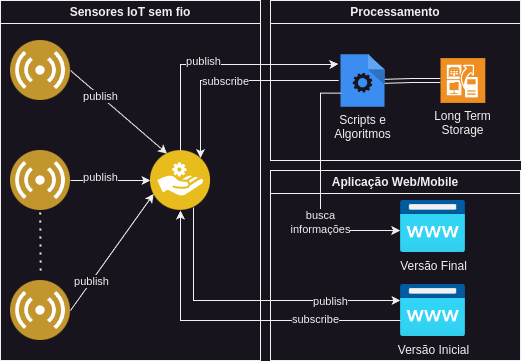
\includegraphics[scale=0.5]{imgs/arquitetura.png}
	\legend{Fonte: Do autor (2024). }
\end{figure}

Observe a diferença do comando $\backslash$includegraphics nas figuras. Na Figura~\ref{fig:figura1} a imagem é configurada para ocupar toda largura da página, enquanto a Figura~\ref{fig:figura2} trabalha escala. Se escala = 1 a figura é mostrada no tamanho original, se escala = 0.5 a figura é mostrada com 50\% do seu tamanho. 

\section{\label{sec:trabRelacionados}Trabalhos relacionados}

O Código~\ref{lst:quadro2} apresenta um trecho de código mágico, escrito na linguagem C++.

\begin{lstlisting}[caption={Exemplo de laço},label={lst:quadro2}]
	void func(int){
	for(int =0;i<10;i++){
		fprintf("asdfas fddfsadf");
	
		}
	}
\end{lstlisting}


\chapter{\label{ch:metodo}Metodologia}
escreva aqui...

\section{\label{sec:arch}Arquitetura}
escreva aqui...

\section{\label{sec:rec}Recursos}
escreva aqui... 

\subsection{\label{sec:cronos}Cronograma}
escreva aqui...

*** importante, conforme a ABNT o cronograma não é uma Tabela - quadro apenas quadro.

O Quadro~\ref{cronoQuinzenal} mostra um formato de cronograma quinzenal, com as atividades escritas diretamente no quadro, já o Quadro~\ref{cronoSemanal} mostra um formato de cronograma semanal.

\begin{quadro}[htb]
	\smaller
	\caption{\label{cronoQuinzenal}Quadro com formato de cronograma quinzenal.}	
	\begin{tabu}{|X[c 0.25]|X[c 0.5]|X[3]|} \tabucline-
		\textbf{Mês} 	& \textbf{Quinzena}	&	\textbf{Atividade} \\ \tabucline-
		\multirow{2}{*}{Mar}	& 	1 a 15		& ESCREVA AQUI O QUE SERÁ FEITO \\ \tabucline{2-3}
		& 	16 a 30		& ESCREVA AQUI O QUE SERÁ FEITO    \\ \tabucline-
		\multirow{2}{*}{Abr}	& 	1 a 15		& ESCREVA AQUI O QUE SERÁ FEITO    \\ \tabucline{2-3}
		& 	16 a 30		& ESCREVA AQUI O QUE SERÁ FEITO    \\ \tabucline-
		\multirow{2}{*}{Mai}	& 	1 a 15		& ESCREVA AQUI O QUE SERÁ FEITO    \\ \tabucline{2-3}
		& 	16 a 30		& ESCREVA AQUI O QUE SERÁ FEITO    \\ \tabucline-
		\multirow{2}{*}{Jun}	& 	1 a 15		& ESCREVA AQUI O QUE SERÁ FEITO    \\ \tabucline{2-3}
		& 	16 a 30		& ESCREVA AQUI O QUE SERÁ FEITO    \\ \tabucline-
		\multirow{2}{*}{Jul}	& 	1 a 15		& ESCREVA AQUI O QUE SERÁ FEITO    \\ \tabucline{2-3}
		& 	16 a 30		& ESCREVA AQUI O QUE SERÁ FEITO    \\ \tabucline-
		\multirow{2}{*}{Ago}	& 	1 a 15		& ESCREVA AQUI O QUE SERÁ FEITO    \\ \tabucline{2-3}
		& 	16 a 30		& ESCREVA AQUI O QUE SERÁ FEITO    \\ \tabucline-		
	\end{tabu}
\end{quadro}


\begin{quadro}[htb]
	\smaller
	\caption{\label{cronoSemanal}Quadro com formato de cronograma semanal.}	
	\begin{tabu}{|X[c 0.25]|X[c 0.5]|X[3]|} \tabucline-
		\textbf{Mês} 	& \textbf{Quinzena}	&	\textbf{Atividade} \\ \tabucline-
		\multirow{4}{*}{Mar}	& 	1 		& atividades da semana  			\\ \tabucline{2-3}
								& 	2		& atividades da semana 		    \\ \tabucline{2-3}
								& 	3		& atividades da semana 		    \\ \tabucline{2-3}
								& 	4		& atividades da semana 		    \\ \tabucline-
		\multirow{4}{*}{Abr}	& 	1 		& atividades da semana  			\\ \tabucline{2-3}
								& 	2		& atividades da semana 		    \\ \tabucline{2-3}
								& 	3		& atividades da semana 		    \\ \tabucline{2-3}
								& 	4		& atividades da semana 		    \\ \tabucline-
		\multirow{4}{*}{...}	& 	1 		& atividades da semana  			\\ \tabucline{2-3}
								& 	2		& atividades da semana 		    \\ \tabucline{2-3}
								& 	3		& atividades da semana 		    \\ \tabucline{2-3}
								& 	4		& atividades da semana 		    \\ \tabucline-
	\end{tabu}
\end{quadro}


O Quadro~\ref{cronGantt} apresenta um cronograma no formato semanal, do tipo Gráfico de Gantt, onde vamos marcando a semana em que determinada atividade será feita. Neste formato a atividade não vai escrita no quadro, sendo necessário ter uma lista numerada (conforme abaixo) detalhando as atividades previstas no projeto. 

As ações necessárias para a execução do projeto são:
\begin{enumerate}
	\item ação 1;
	\item ação 2;
	\item outra ação;
	\item ....
	\item última ação.
\end{enumerate}

\begin{quadro}[htb]
	\smaller
	\caption{\label{cronGantt}Quadro com formato de cronograma semanal.}	
	\begin{tabu}{|X[c 2]|X[c 0.25]|X[c 0.25]|X[c 0.25]|X[c 0.25]|X[c 0.25]|X[c 0.25]|X[c 0.25]|X[c 0.25]|X[c 0.25]|X[c 0.25]|X[c 0.25]|X[c 0.25]|X[c 0.25]|X[c 0.25]|X[c 0.25]|X[c 0.25]|X[c 0.25]|X[c 0.25]|X[c 0.25]|X[c 0.25]|} \tabucline-
		\rowcolor{gray} 	& \multicolumn{4}{c|}{\textbf{Mar}} & \multicolumn{4}{c|}{\textbf{Abr}}& \multicolumn{4}{c|}{\textbf{Mai}}& \multicolumn{4}{c|}{\textbf{Jun}}& \multicolumn{4}{c|}{\textbf{Jul}} 	\\ \tabucline-
		Ação	& 1 & 2 & 3 & 4 & 1 & 2 & 3 & 4 & 1 & 2 & 3 & 4 & 1 & 2 & 3 & 4 & 1 & 2 & 3 & 4   \\ \tabucline-
		1	& x & x & &  &  &  &  &  &  &  &  &  &  &  &  &  &  &  &  &   \\ \tabucline-
		2	&  & x & x &  &  &  &  &  &  &  &  &  &  &  &  &  &  &  &  &   \\ \tabucline-
	3	&  &  & x & x  &  &  &  &  & x & x &  &  &  &  &  &  &  &  &  & \\ \tabucline-
	\end{tabu}
\end{quadro}

Para editar no latex, basta copiar a última linha, colocar o número certo e marcar com X no quadrinho desejado. Por exemplo, vamos definir que a atividade 3 será executada nas semanas 3 e 4 de Março e novamente nas semanas 1 e 2 de Maio.  Para tanto, inserimos 'x' a direita do terceiro, quarto, décimo e décimo primeiro \&s. 

Os símbolos \& precisam apenas estar em quantidade certa, sem precisar estar alinhados.

\begin{verbatim}
	3	&  &  & x & x  &  &  &  &  &  & x & x &  &  &  &  &  &  &  &  & \\ \tabucline-
\end{verbatim}

